\documentclass{beamer}
%\usepackage{media9} 
\usepackage[english]{babel}
\usepackage{times}
\usepackage{graphicx}
\usepackage{amsmath}
\usepackage{movie15}
\usepackage{hyperref}

%\usepackage{hyperref}
\usepackage{listings}
\usepackage{hhline}
\usepackage{pifont}
\usepackage{amssymb}
\usepackage{color, colortbl}

\lstset{language=C++,
columns=fullflexible,
keepspaces=true,
breaklines=true,
tabsize=3,
showstringspaces=false,
extendedchars=true,
breakatwhitespace=true}

%
% Choose how your presentation looks.
%
% For more themes, color themes and font themes, see:
% http://deic.uab.es/~iblanes/beamer_gallery/index_by_theme.html
%
\mode<presentation>
{
	\useinnertheme[shadow=true]{rounded}
	\useoutertheme{infolines}
	\usecolortheme{whale}
	
	\setbeamersize{text margin left=1em,text margin right=1em}
	\setbeamercolor{titlelike}{parent=structure,bg=lightgray!10!white}
    \setbeamercovered{transparent}
}

\AtBeginSection[]
{
  \begin{frame}<beamer>
  \frametitle{Outline}
  \tableofcontents[currentsection]
  \end{frame}
}


\title[Local Time Stepping]{HPC-LEAP Workshop:\\ Shallow Water Equation for Tsunami Simulation} 
\subtitle{Local Time Stepping}

\author[Xiao Xue, Andrew Brockman]{Xiao Xue, Andrew Brockman}  % (optional, use only with lots of authors)
\institute[]{HPC-LEAP Marie Curie Action}
\date{30 June 2016}

\begin{document}
\begin{frame}
  \titlepage
\end{frame}

% Uncomment these lines for an automatically generated outline.
\begin{frame}{Outline}
  \tableofcontents
\end{frame}

\section{Introduction}
\begin{frame}[t]{2004 Indian Earthquake Tsunami}
  \begin{figure}[p]
    \centering
    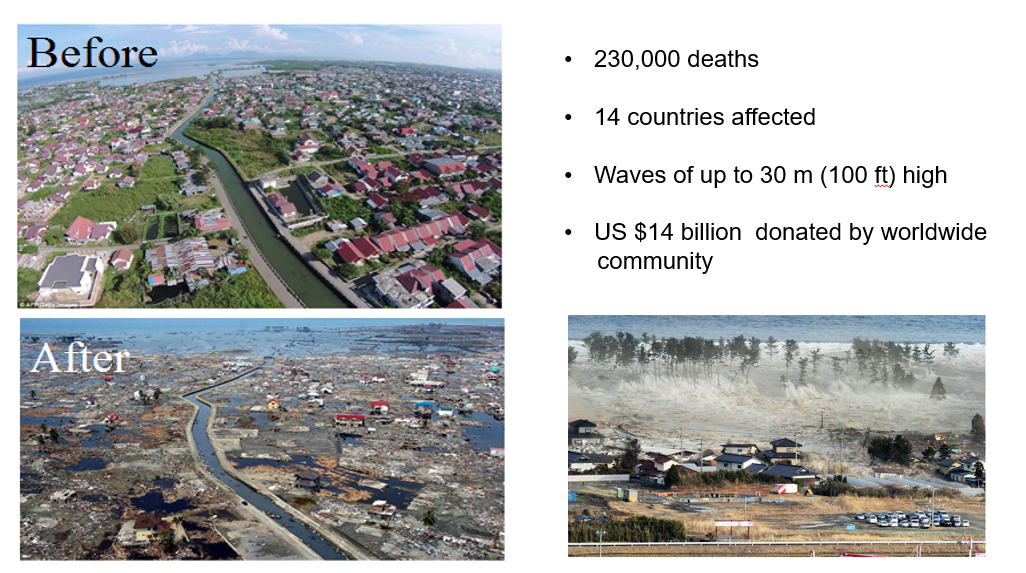
\includegraphics[width=\textwidth]{tsunami}
    %\caption{Norm difference of GTS \& LTS with different different time step($L=3$)}
    \label{fig:awesome_image}
\end{figure}
\end{frame}

%Algorithms frame started
\section{Numerical Scheme for Shallow Water Equations}
\subsection{1D SWE}
% Algorithms-Meacurvature
\begin{frame}{1D shallow water equations}

    \begin{block}{1D shallow water equations}
      \begin{itemize}
        \item $h(x,t)$ is the fuild depth, $u(x,t)$ is the fluid velocity,$g$ is the gravity constant,$B(x)$ is relative to sea level.
        
      \end{itemize}
      \begin{center}
      	$h_{t} + (hu)_{x} = 0$,\\
	    $(hu)_{t} + (hu^{2} + \frac{1}{2}gh^{2})_{x} \alert{+ ghB_{x}} =0$
	  \end{center}
    \end{block}
  
 
\end{frame}
% 2D shallow water equations
\subsection{2D SWE}
\begin{frame}{2D shallow water equations}

	\begin{block}{2D shallow water equations}
      \begin{itemize}
        \item $h(x,y,t)$ is the fuild depth, $u(x,t)$ and $v(y,t)$ are fluid velocity in two different directions,$g$ is the gravity constant,$B(x,y)$ is relative to sea level.
        
      \end{itemize}
      \begin{center}
      	$h_{t} + (hu)_{x} + (hu)_{y} = 0$,\\
$(hu)_{t} + (hu^{2} + \frac{1}{2}gh^{2})_{x}+(huv)_{y} + \alert{ghB_{x}} =0$,\\
$(hv)_{t} +(huv)_{x} + (hv^{2} + \frac{1}{2}gh^{2})_{y}+ \alert{ghB_{y}}=0$,\\
	  \end{center}
    \end{block}

\end{frame}

\subsection{Godunov \& Roe solver} % keep it simple
\begin{frame}{Godunov \& Roe solver}
\begin{block}{Godunov's Method}
  \begin{itemize}
    \item Recall $Q_{i}$ represents the average of $q(x,t_{n})$ over cell $C_{i}$
     \begin{center}
    $Q_{i}^{n} \approx \frac{1}{\Delta x}\int_{x_{i-\frac{1}{2}}}^{x_{i+\frac{1}{2}}}q(x,t_{n})dx$
    \end{center}
    \item Godunov's method can be represent as follow, detail in [2,p.311]
         \begin{center}
    $Q_{i}^{n+1} = Q_{i}^{n}  - \frac{\Delta t}{\Delta x}(F_{i+\frac{1}{2}}^{n} - F_{i-\frac{1}{2}}^{n})$
    with $F_{i + \frac{1}{2}}^{n} =\boldsymbol{F}(Q_{i+1},Q_{i})$
        \end{center}

  \end{itemize}
\end{block}
\end{frame}
% formula for world
\begin{frame}{Godunov \& Roe solver}

  \begin{block}{Roe Approximation}
	\begin{itemize}
	\item Roe's Riemann solver approximation is linearize the nonlinear problem $q_{t}+f(q)_{x}=0$ to
         \begin{center}
    $\hat{q_{t}}+\hat{A_{i-1/2}}\hat{q_{x}}=0$
        \end{center}
        The matrix $\hat{A_{i-1/2}}$ is chosen to be some approximation to $f^{'}(q)_{x}$ valid in a neighborhood of $Q_{i-1}$ and $Q_{i}$
    \item Roe Approximation:\\
    \begin{center}
    $\hat{q}=\begin{bmatrix}
\hat{h}\\ 
\hat{h}\hat{u}
\end{bmatrix}$
    \end{center}
    where \\\begin{center}$\hat{h}=\frac{h_{l}+h_{r}}{2}$, and $\hat{u}=\frac{u_{l}\sqrt{h_{l}}+u_{r}\sqrt{h_{r}}}{\sqrt{h_{l}} + \sqrt{h_{r}}}$ \end{center}

  \end{itemize}

  \end{block}

\end{frame}

% Algorithms frame ended
% CUDA Implementation & Optimization
\section{Local Time Stepping Scheme}
\subsection{Hierarchical scheme}
% Memory Allocation Optimization
\begin{frame}[t]{Hierarchical LTS Scheme}
\only<2->{
  \begin{block}{Continue: Godunov \& Roe solver}
    \begin{itemize}
      \item The Godunov \& Roe solver previously introduced is worked on the GTS where \alert{$\Delta t$} is constant at each loop.
      \begin{center}
    $Q_{i}^{n+1} = Q_{i}^{n}  - \frac{\alert{\Delta t}}{\Delta x_{i}}(F_{i+\frac{1}{2}}^{n} - F_{i-\frac{1}{2}}^{n})$
    \end{center}
    \item \alert{$\Delta t$} will be limited by \textit{CFL condition}: $\alert{\Delta t} \leq C_{max}min{(\frac{\Delta x_{i}}{U_{i}})}$
    \end{itemize}
    
  \end{block}
}
\only<3->{
	\begin{block}{Solution: LTS}
    \begin{itemize}
      \item Use $\Delta t_{i}$ locally, to avoid the unnecessary calculation.
      \item \alert{Question:}\\ How to synchronize with different time step per cell?
    \end{itemize}
  \end{block}
}

\end{frame}
\begin{frame}[t]{Hierarchical LTS Scheme}
\begin{block}{General equation of LTS}
    \begin{itemize}
      \item Most part remain the same with GLS scheme instead of $\Delta t_{i}$
      \begin{center}
      $Q_{i}^{n+1} = Q_{i}^{n}  - \frac{\alert{\Delta t_{i}}}{\Delta x_{i}}(F_{i+\frac{1}{2}}^{n} - F_{i-\frac{1}{2}}^{n})$
      \end{center}
      Where $\Delta t_{i}$ is equal to $2^{l-1}\Delta t_{min}$. $\Delta t_{min}$ is the minum time step calculated by GTS. $l$ is the interger of pre-set level for each cell. 
    \end{itemize}
  \end{block}
\end{frame}

\subsection{Local CFL Condition}
\begin{frame}[t]{Local CFL Condition}
\begin{block}{Local Courant Number}
    \begin{itemize}
      \item A preliminary cell-based LTS level $l_{c}$ is assigned to cell $i$ according to the local Courant number $Cr_{i}$ computed as
      \begin{center}
      $Cr_{i} = \frac{\Delta t_{min}}{\Delta x_{i}}max_{k=1,2}(u_{k})$
      \end{center}
      Where $u_{k}$ is the cell wave speed on one of 2 directions.
    \end{itemize}
\end{block}
\end{frame}

\begin{frame}[t]{Local CFL Condition}
\begin{block}{Local Time Step Level Criterion}
    \begin{itemize}
      \item After calculated the local Courant number the local time step level is determined by
      \begin{center}
      $Cr_{0}/2^{l-1}\leq Cr_{i}< Cr_{0}/2^{l-2}$
      \end{center}
      with the exception of level 1 which is controlled by $Cr_{i}> Cr_{i}/2$. $Cr_{0}$ is the maximum courant number for the simulation.
    \end{itemize}
  \end{block}
\end{frame}
% add buffer cell part
\begin{frame}{Hierarchical LTS Scheme: illustration}
\begin{figure}[p]
    \centering
    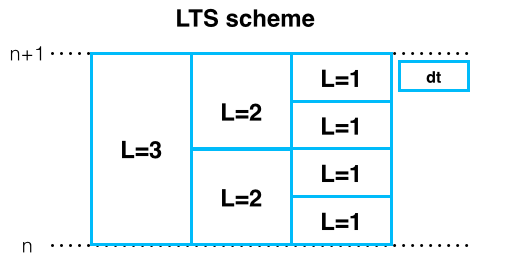
\includegraphics[width=1\textwidth]{LTS_scheme}
    \caption{LTS scheme: first look}
    \label{fig:awesome_image}
\end{figure}
\end{frame}
\begin{frame}{Hierarchical LTS Scheme: illustration}
\begin{figure}[p]
    \centering
    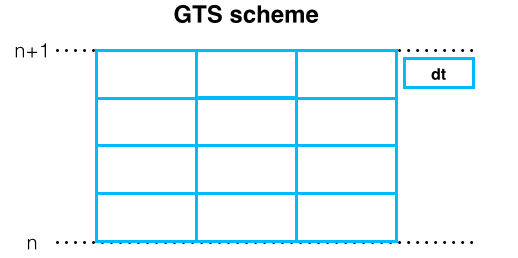
\includegraphics[width=1\textwidth]{GTS_scheme}
    \caption{GTS scheme: computational over head}
    \label{fig:awesome_image}
\end{figure}
\end{frame}
\begin{frame}{Hierarchical LTS Scheme: illustration}
\begin{figure}[p]
    \centering
    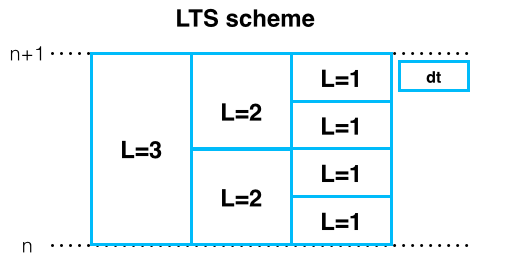
\includegraphics[width=1\textwidth]{LTS_scheme}
    \caption{LTS scheme: benefit}
    \label{fig:image}
\end{figure}
\end{frame}
\begin{frame}{Hierarchical LTS Scheme: illustration}
\begin{figure}[p]
    \centering
    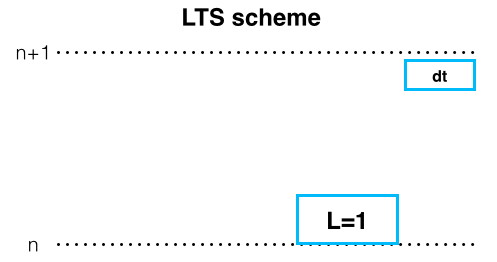
\includegraphics[width=1\textwidth]{LTS_T1}
    \caption{Local cell update: initial step}
    \label{fig:some_image}
\end{figure}
\end{frame}
\begin{frame}{Hierarchical LTS Scheme: illustration}
\begin{figure}[p]
    \centering
    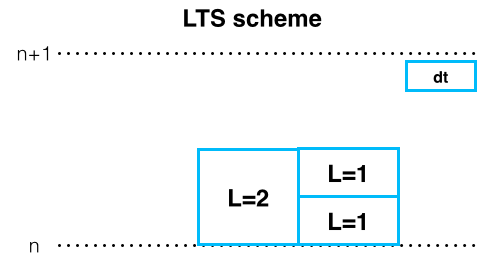
\includegraphics[width=1\textwidth]{LTS_T2}
    \caption{Local cell update: step 2}
    \label{fig:awe}
\end{figure}
\end{frame}
\begin{frame}{Hierarchical LTS Scheme: illustration}
\begin{figure}[p]
    \centering
    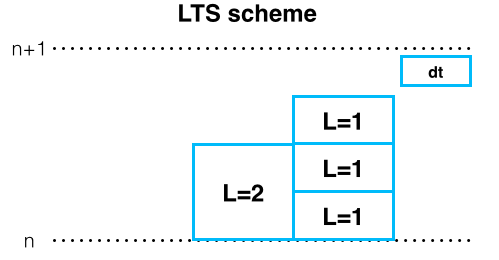
\includegraphics[width=1\textwidth]{LTS_T3}
    \caption{Local cell update: step 3}
    \label{fig:awesome_img}
\end{figure}
\end{frame}
\begin{frame}{Hierarchical LTS Scheme: illustration}
\begin{figure}[p]
    \centering
    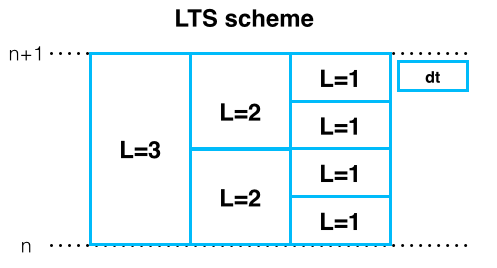
\includegraphics[width=1\textwidth]{LTS_T4}
    \caption{Local cell update: step 4}
    \label{fig:awesome}
\end{figure}
\end{frame}

%\begin{frame}{Summery for LTS}
%\begin{itemize}
 %     \item Advantages: improve computation efficiency without loosing accuracy
      
%      \item Disadvantages: may have unstable cases near shock wave boundary
%    \end{itemize}
%\end{frame}
% \subsection{Other schemes}
% \begin{frame}[fragile,t]
	
% 	}
% \end{frame}

\section{Result \& Animation}
\subsection{Shallow Water Equations}
\begin{frame}{1D SWE \& LTS vs. GTS}
\begin{itemize}
\item The experienment is based on breaking dam scheme in 1D shallow water equations(GTS scheme - timestep 200)\\
\end{itemize}
\begin{center}
\includemovie[
   poster,controls,
   text={\small(Loading)}
 ]{6cm}{6cm}{swe1D_GTS.mov}
%\includemovie[poster,controls, text={\small(swe1D_LTS_mov.mov)}]{6cm}{6cm}{swe1D_LTS_mov.mov}
\end{center}
\end{frame}
\begin{frame}{1D SWE \& LTS vs. GTS}
\begin{itemize}
\item The experienment is based on breaking dam scheme in 1D shallow water equations(LTS scheme - timestep 200)\\
\end{itemize}
\begin{center}
\includemovie[
   poster,controls,
   text={\small(Loading)}
 ]{8cm}{6cm}{swe1D_LTSscheme.mov}
%\includemovie[poster,controls, text={\small(swe1D_LTS_mov.mov)}]{6cm}{6cm}{swe1D_LTS_mov.mov}
\end{center}
\end{frame}
\begin{frame}{2D SWE \& LTS}
\begin{itemize}
\item The experienment is based on breaking dam scheme in 2D shallow water equations\\
\begin{center}
\includemovie[
   poster,controls,
   text={\small(Loading)}
 ]{8cm}{6cm}{swe2D_waterhight.mov}
\end{center}
\end{itemize}
\begin{center}
\end{center}
\end{frame}
\begin{frame}{2D SWE \& LTS}
\begin{itemize}
\item The experienment is based on breaking dam scheme in 2D shallow water equations\\
\begin{center}
\includemovie[
   poster,controls,
   text={\small(Loading celldt.mov)}
 ]{8cm}{6cm}{swe2D_dtcell.mov}
\end{center}
\end{itemize}
\begin{center}
\end{center}
\end{frame}
\subsection{Accuracy}
\begin{frame}[t]{2D SWE LTS Error Measurement}
  \begin{block}{Experienmental Environment}
        \begin{itemize}
            \item Domain size: 50 by 50
            \item Error measurement is using the norm formula in compare with GTS\\
            \begin{center}
            	$E_{2}(d_{LTS}) = (\sum_{i=1,...,N}^{ }[(d_{LTS})_{i} - d_{GTS})_{i}]^{2})^{1/2}$
            \end{center}
        \end{itemize}
    \end{block}
\end{frame}
\begin{frame}{2D SWE LTS Error Measurement}
%graph for runtime from 100 - 2000 time step
\begin{figure}[p]
    \centering
    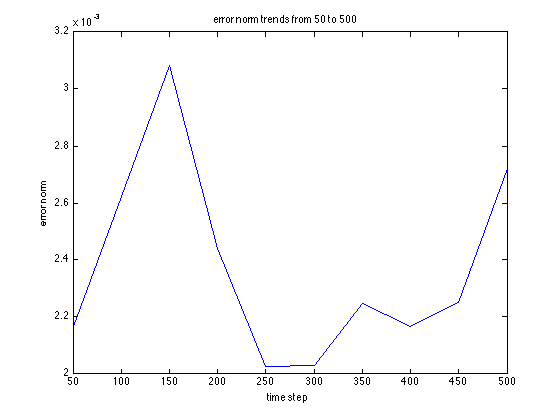
\includegraphics[width=0.6\textwidth]{2d_lts_error}
    \caption{Norm difference of GTS \& LTS with different different time step($L=3$)}
    \label{fig:awesome_image}
\end{figure}
\end{frame}
\subsection{Benchmark}
\begin{frame}{Benchmark}
%graph for runtime from 100 - 2000 time step
\begin{figure}[p]
    \centering
    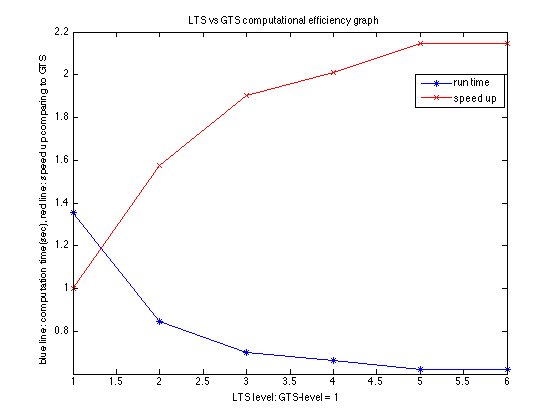
\includegraphics[width=0.6\textwidth]{LTS_runtime}
    \caption{graph showed runtime difference of GTS \& LTS with different LTS levels(1000 time steps)}
    \label{fig:awesome_image}
\end{figure}
\end{frame}
\subsection{MPI Speedup}
\begin{frame}{MPI parallelization}
%graph for runtime from 100 - 2000 time step
\begin{figure}[p]
    \centering
    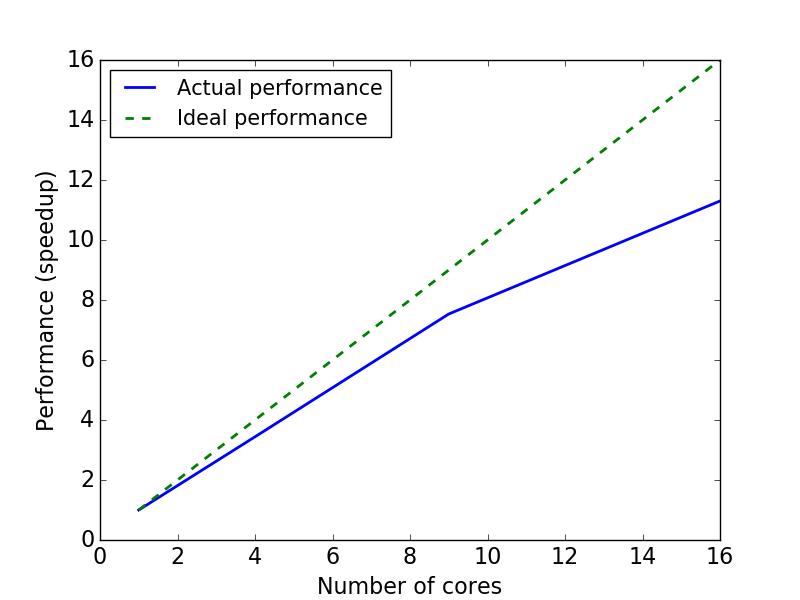
\includegraphics[width=0.8\textwidth]{mpi_peformance}
    %\caption{Norm difference of GTS \& LTS with different different time step($L=3$)}
    \label{fig:awesome_image}
\end{figure}
\end{frame}

\section[]{References}

\begin{frame}[t]{References:}
[1]R.J. LeVeque. Finite Volume Methods for Hyperbolic Problems. Cambridge Texts in Applied Mathematics. Cambridge University Press, 2002
    
[2] R.J.LeVeque, D.L.George, M.J.Berger. Tsunami modelling with adaptively refined finite volume methods. Acta Numerica, pp.211 - 289, 2011

[3] Bradford, S.F. and Sanders, B.F., Finite-Volume Model for Shallow-Water Flooding of Arbitrary Topography, ASCE Journal of Hydraulic Engineering. 128(3), 289-298, 2002.

[4] Crossley, A.J., Wright, N.G., Whitlow, C.D. Local time stepping for modeling open channel flows. J. Hydr. Engng.129(6), 455–462, 2003

[5]Osher, S., Sanders, R. Numerical approximations to nonlinear conservation laws with local varying time and space grids. Mathematics of Computation 41(164), 321–336,1983.
\end{frame}

\section*{Thanks}

\begin{frame}[t]{Thanks for your attention! Questions?}

\end{frame}

\end{document}
